\documentclass[tikz,border=5pt]{standalone}

\usepackage{tikz}

\begin{document}

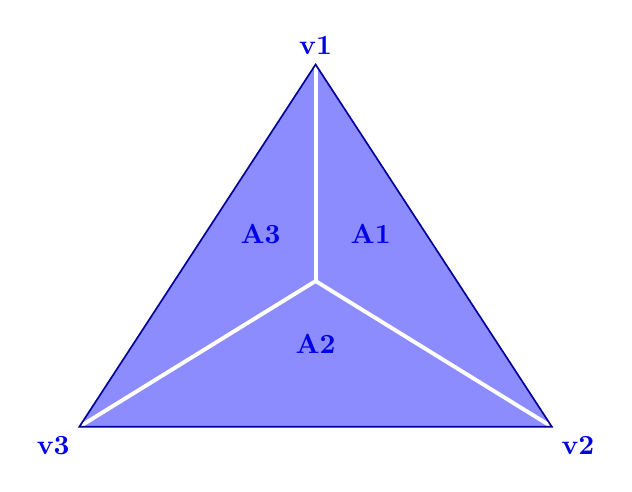
\begin{tikzpicture}
\coordinate (v3) at (0,0);
\coordinate (v2) at (6,0);
\coordinate (v1) at (3,4.6);
\coordinate (C)  at (3,1.85);

\fill[blue!45] (v3) -- (v2) -- (v1) -- cycle;

\draw[white, line width=1.4pt] (C) -- (v1);
\draw[white, line width=1.4pt] (C) -- (v2);
\draw[white, line width=1.4pt] (C) -- (v3);

\draw[blue!60!black, line width=0.6pt] (v3) -- (v2) -- (v1) -- cycle;

\node[blue!90!black, font=\bfseries] at (3.7,2.45) {A1};
\node[blue!90!black, font=\bfseries] at (3.0,1.05) {A2};
\node[blue!90!black, font=\bfseries] at (2.3,2.45) {A3};

\node[blue!90!black, font=\bfseries] at (v1) [above] {v1};
\node[blue!90!black, font=\bfseries] at (v2) [below right] {v2};
\node[blue!90!black, font=\bfseries] at (v3) [below left] {v3};
\end{tikzpicture}

\end{document}
